% !TEX root = ../thesis.tex

\chapter{Vizualizácia genómu SARS-CoV-2}

Táto kapitola je zameraná na použitie niektorých postupov vizualizácie 2D genómu na genóm SARS-CoV-2.
Pretože téma je mimoriadne zložitá, sú predstavené iba niektoré z existujúcich metód.
Komplexný prehľad týchto metódach, ich analýza a implementácia je obsiahnutá v zodpovedajúcich sekcíach.

Druhá časť tejto kapitoly je zameraná na zostavenie funkčného softvéru, ktorý je schopný vizualizovať genóm SARS-CoV-2 pomocou predtým popísaných techník a knižníc.

\section{FASTA, GFF a GBK formaty}

Najskôr, pochopenie toho, ako sa genomické údaje ukladajú, je kľúčom ku správnej vizualizácii.
Možné riešenia vizualizácie možno všeobecne rozdeliť do dvoch samostatných kategórií: tie, ktoré používajú samotnú sekvenciu genómu, a tie, ktoré používajú anotácie genómu \cite{covvisual}.

Prvá kategória funguje na sekvencii surovej DNA (RNA) a zvyčajne sa používa na hľadanie rôznych vzorov, tandemových opakovaní, bodových mutácií alebo na vizuálne porovnanie genómov príbuzných druhov.
Prvotné údaje, buď DNA, alebo aminokyselinové sekvencie, sa zvyčajne ukladajú vo formáte FASTA (prípony súborov .fasta, .fa, .fna)\cite{fasta}.

Zdrojový kód uvedený nižšie demonštruje štruktúru súboru FASTA obsahujúceho sekvenciu DNA SARS-CoV-2.

\begin{lstlisting}[caption={Prvých 180 nukleotidov z genómovej sekvencie SARS-CoV-2 vo formáte FASTA. Riadok popisu, ktorý sa začína znakom „>“, obsahuje informácie o postupnosti. Za začiatočným riadkom je samotná aktuálna sekvencia v štandardnom jednopísmenovom reťazci znakov.},captionpos=b]
  >NC_045512.2 |Coronavirus 2 isolate Wuhan-Hu-1, complete genome
  ATTAAAGGTTTATACCTTCCCAGGTAACAAACCAACCAACTTTCGATCTCTTGTAGATCT
  GTTCTCTAAACGAACTTTAAAATCTGTGTGGCTGTCACTCGGCTGCATGCTTAGTGCACT
  CACGCAGTATAATTAATAACTAATTACTGTCGTTGACAGGACACGAGTAACTCGTCTATC
\end{lstlisting}


Druhá kategória medzitým používa predspracované a dobre preštudované údaje \cites{gff}, ktoré sú získané zo surovej sekvencie.
Anotácie genómu obsahujú miesta kódujúcich oblastí genómu, a preto môžu byť užitočné v oblastiach spojených s genetikou, syntézou proteínov, dedičnosťou atď.
\begin{figure}[!ht]
	\centering
	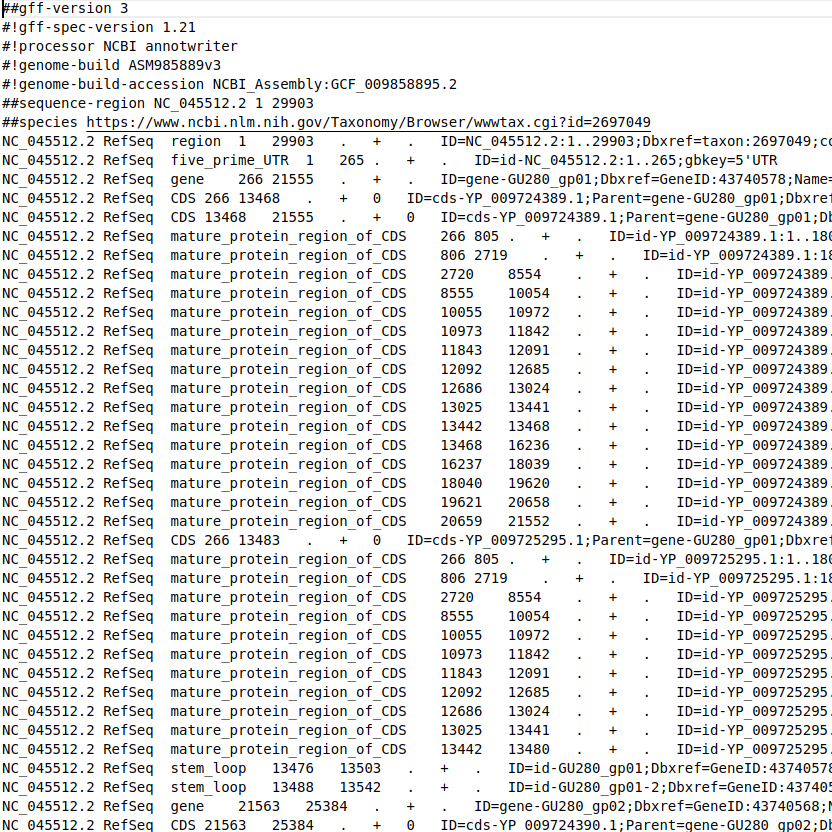
\includegraphics[width=.8\textwidth]{figures/gff3.png}
	\caption{Prvé 45 riadkov anotačného súboru genómu SARS-CoV-2. Pravá časť anotácie je na obrázku skrátená.\label{o:latex_friendly_zone}}
\end{figure}

Každá anotácia genómu má 9 povinných polí:
\begin{enumerate}
    \item ID sekvencie
    \item Zdroj
    \begin{itemize}
        \item Opisuje algoritmus alebo postup, ktorý vygeneroval túto funkciu. Typicky Genescane alebo Genebank
    \end{itemize}
    \item Typ vlastnosťi
    \begin{itemize}
        \item Opisuje, o čo ide (mRNA, doména, exón atď.)
    \end{itemize}
    \item Začiatok vlastnosťi
    \item Koniec vlastnosťi
    \item Skóre 
    \begin{itemize}
        \item Hodnoty podobnosti sekvencií alebo predpovedí
    \end{itemize}
    \item Prameň (+ alebo -)
    \item Fáza
    \begin{itemize}
        \item Označuje, kde vlastnosť začína odkazom na čítací rámec (ORF)
    \end{itemize}
    \item Atribúty
    \begin{itemize}
        \item Zoznam dvojíc značiek a hodnôt oddelených bodkočiarkou, ktorý poskytuje ďalšie informácie o každej funkcii
    \end{itemize}
\end{enumerate}
Tieto údaje sa zvyčajne ukladajú do súborov GFF (General Feature Format). Prípony názvov súborov sú .gff, .gff2. a .gff3 \cite{gff2}.

Okrem anotácií GFF a súborov sekvencií FASTA sa široko používajú aj súbory GBK (formát Genbank).
\begin{figure}[!ht]
	\centering
	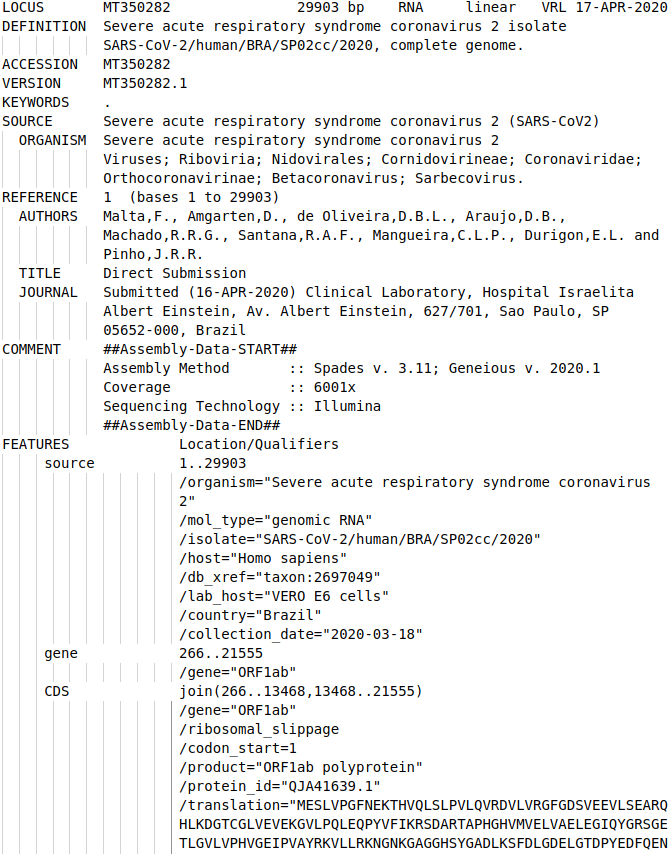
\includegraphics[width=0.7\textwidth]{figures/gbk.png}
	\caption{Prvé 45 riadkov obsahu súboru GBK zodpovedajúcich genómu SARS-CoV-2\label{o:latex_friendly_zone}}
\end{figure}
Formát Genbank umožňuje ukladanie informácií okrem sekvencie DNA / proteínu.
Uchopenie obrazovky zobrazuje rôzne podrobnosti, prvá časť obsahuje LOCUS, DEFINÍCIU, PRÍSTUP a VERZIU záznamu a je označená výrazom PÔVOD, konečným detailom je skutočná postupnosť.
Týchto päť prvkov je podstatnou súčasťou formátu GenBank.

Nepodstatné časti záznamu obsahujú takzvané metaúdaje a môžu obsahovať podrobnejšie informácie o organizme, krížové odkazy na iné databázy a dokonca aj zoznam publikácií, v ktorých je tento záznam uvedený.
Časť záznamu „VLASTNOSTI“ popisuje dôležité charakteristiky sekvencie záznamu, ako je prítomnosť kódujúcich sekvencií, proteínov atď.

\section{Analýza a vizualizácia genómu SARS-CoV-2}
Na vykonanie samotnej analýzy sa použijú balíky BioPython a DNA Features Viewer.

Na vizualizáciu genómu SARS-CoV-2 sú potrebné predtým opísané súbory s genómovými údajmi. 
Súbory FASTA aj GBK je možné získať na webových stránkach NCBI (MN908947).

\subsection{Nucleotides distribution and GC-content}

Analýza sa zvyčajne začína čítaním sekvencie DNA:
\begin{lstlisting}[language=Python, caption=Čítaníe sekvencie DNA pomocou BioPython:]
    from Bio.SeqRecord import SeqRecord
    from Bio import SeqIO
    cov19 = SeqIO.read('MN908947.fna', "fasta")
\end{lstlisting}

Jednou z najdôležitejších genomických vlastností je GC-content (alebo obsah guanín-cytozínu) \cite{gccontent2}.
Je to percento dusíkatých báz v molekule DNA alebo RNA, ktoré sú buď guanín (G) alebo cytozín (C).
Toto opatrenie udáva podiel báz G a C z implikovaných štyroch celkových báz, tiež zahŕňajúcich adenín a tymín v DNA a adenín a uracil v RNA.

Obsah GC sa môže uviesť pre určitý fragment DNA alebo RNA alebo pre celý genóm.
Ak sa jedná o fragment, môže to znamenať obsah GC v individuálnom géne alebo časti génu (doméne), skupine génov alebo génových zhlukov alebo nekódujúcej oblasti \cite{gccontent}.

Obsah GC sa zvyčajne vyjadruje ako percentuálna hodnota, niekedy však ako pomer.
Percento obsahu GC sa počíta ako:

    \[\frac{G+C}{A+T+G+C}*100\%\]

    Distribúciu nukleotidov (A, T, C, G) v DNA Covid19 je možné vypočítať pomocou priloženého kódu.
\begin{lstlisting}[language=Python, caption=Skript na výpočet distribúcie nukleotidov v genóme SARS-CoV-2.]
    #Count the nucleotides frequency in the DNA
    DNA = SARS_Cov_2_DNA
    nucleotides = {}
    for n in DNA:
        if n in nucleotides:
            nucleotides[n] += 1
        else:
            nucleotides[n] = 1

    #Create a dataframe
    nts = pd.DataFrame(data=nucleotides, 
                                index=[0]).T.reset_index()
    nts = nts.rename(columns={0: 'frequency', 
                                'index': 'nucleotides'})
    nts = nts.sort_values(by=['frequency'], ascending=True)
\end{lstlisting}

Prvým pozorovaním je, že frekvencia nukleotidov A (8954) a T (9594) je vyššia ako frekvencia C (5492) a G (5863).
Preto je obsah GC 37,97\%.
Pri komparácii môže byť obsah GC v eukaryotoch, ako sú stavovce, vrátane ľudí, až 60\% \cite{gccontent3}.

\begin{figure}[!ht]
	\centering
	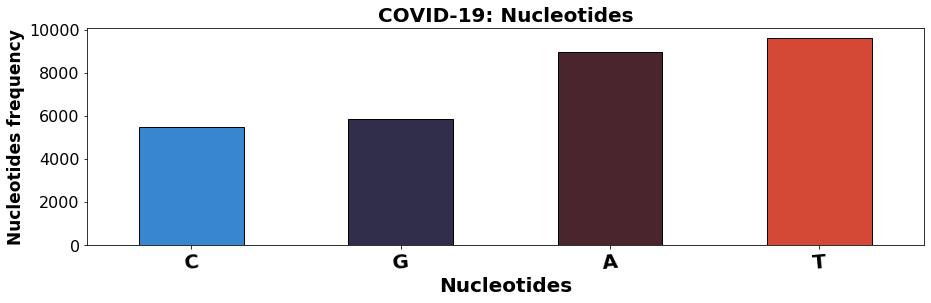
\includegraphics[width=0.9\textwidth]{figures/covidnucleotides.png}
	\caption{Diagrama ukazujúca distribúciu SARS-CoV-2 nukleotidov.\label{o:latex_friendly_zone}}
\end{figure}

\subsection{Gatesova metóda}
2D metódy sú primárne založené na karteziánskom súradnicovom systéme a samotnou reprezentáciou je sada bodiek alebo vektorov zodpovedajúcich rôznym vlastnostiam genómu;
Gatesova metóda je typickým príkladom 2D vizualizačných techník, ktoré pracujú so surovými genomickými dátami.
Preto sa počas vizualizácie spracováva súbor FASTA.

Je to pochopiteľné a bol som vybraný ako jeden z metód na implementáciu, pretože som ho omylom znovu objavil pri tvorbe bakalárskej práce.

Štyri bázy nukleových kyselín sú priradené k štyrom osiam 2D karteziánskeho súradnicového systému.
Daná sekvencia sa vynesie do grafu podľa distribúcie jej báz v príslušnom smere;
vo výpočtoch je adenín (A) priradený k negatívnej osi x, cytozín (C) k pozitívnej osi y, guanín (G) k pozitívnej osi x a tymín (T) k negatívnej osi y.
Vážený priemer súradníc x a y každého bodu sekvencie dĺžky N predstavuje ťažisko.
Euklidovská vzdialenosť medzi začiatkom a centrom hmoty poskytuje kvantitatívny deskriptor grafu, ktorý sa nazýva polomer grafu.

Táto metóda môže byť použitá na hľadanie podobností medzi príbuznými genómami a na hľadanie vzorov v konkrétnych.
Napríklad po vizualizácii sekvencie genómu SARS-CoV-2 pomocou Gatesovej metódy je sekvencia 33 adenínových (červených) nukleotidov ľahko rozlíšiteľná v celom genóme.
\begin{figure}[!ht]
	\centering
	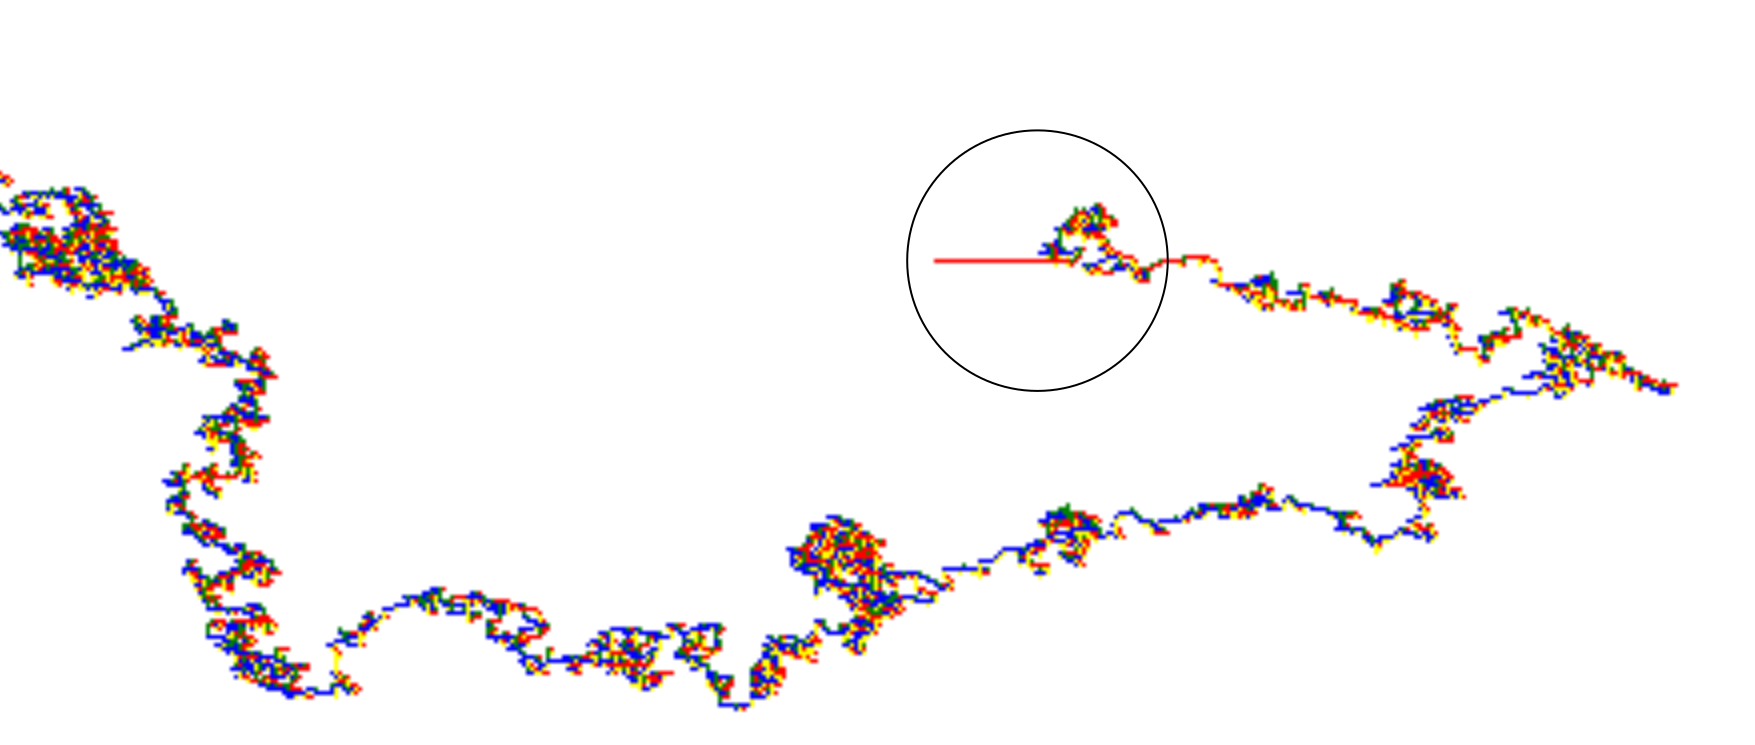
\includegraphics[width=0.6\textwidth]{figures/aaaaa.png}
	\caption{Časť reprezentácie genómu SARS-CoV-2 pomocou Gatesovej metódy. Dlhá sekvencia 33 adenínových nukleotidov je označená čiernym kruhom.\label{o:latex_friendly_zone}}
\end{figure}

Po vyšetrení súboru FASTA môžeme vidieť, že na samom konci sekvencie genómu je 33 adenínových nukleotidov, ako je uvedené nižšie (obr. 2.5).

\begin{figure}[!ht]
	\centering
	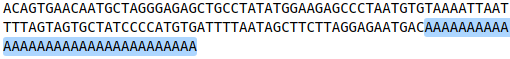
\includegraphics[width=0.7\textwidth]{figures/AAAA.png}
	\caption{Posledné 143 nukleotidy genómu vírusu SARS-CoV-2 v súbore FASTA so sekvenovaným genómom. Je zvýraznená dlhá sekvencia 33 adenínových nukleotidov.\label{o:latex_friendly_zone}}
\end{figure}

Ďalším príkladom nájdenia vzorov v sekvencii DNA pomocou Gatesovej metódy je pokus o vizualizáciu nukleotidovej sekvencie prvého chromozómu \textit{Encephalitozoon Intestinalis}, ktorý sa považuje za najmenší eukaryotický genóm \cite{smalleu}.
Sekvenciu je možné ľahko získať pomocou zdrojov NCBI (ID CP001942).

Po vizualizácii spomínaného chromozómu je prvým pozorovaním to, že obidva konce sekvencie sú takmer identické (obr. 2.6).
Jediný rozdiel, s výnimkou bodových mutácií, je ten, že sú zložené z nukleotidov komplementu.
Preto to možno považovať za dôkaz použiteľnosti metódy pri vyhľadávaní vzorov.

\begin{figure}[!ht]
	\centering
	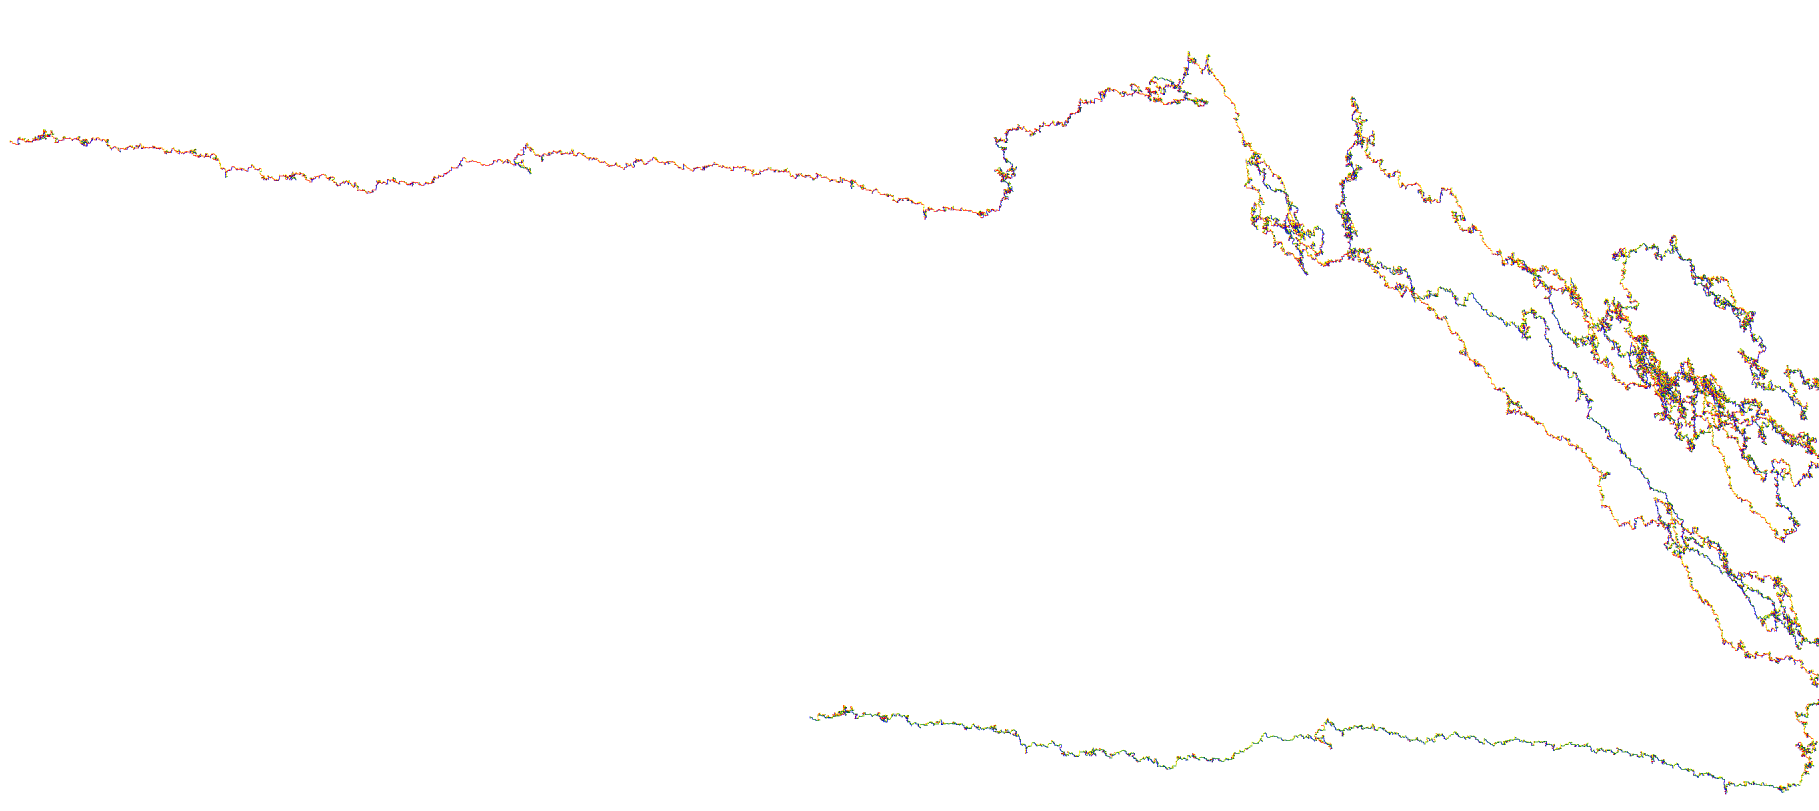
\includegraphics[width=0.7\textwidth]{figures/gateseu.png}
	\caption{Časť prvej vizualizácie chromozómu Encephalitozoon Intestinalis. Rovnaké sekvencie sú zobrazené v strede.\label{o:latex_friendly_zone}}
\end{figure}

Najbližším príbuzným moderného vírusu + ssRNA SARS-CoV-2 je vírus SARS-CoV, ktorý bol príčinou vypuknutia SARS v roku 2004 \cite{cov1cov2}.
Za jasný príklad použitia tejto metódy možno považovať komprimáciu sekvencií genómu SARS-CoV a SARS-CoV-2.

Samotný rozruch je možné vykonať pomocou Squiggle, dvojrozmernej knižnice vizualizácie sekvencií DNA \cite{Lee2018}.
\begin{figure}[!ht]
	\centering
	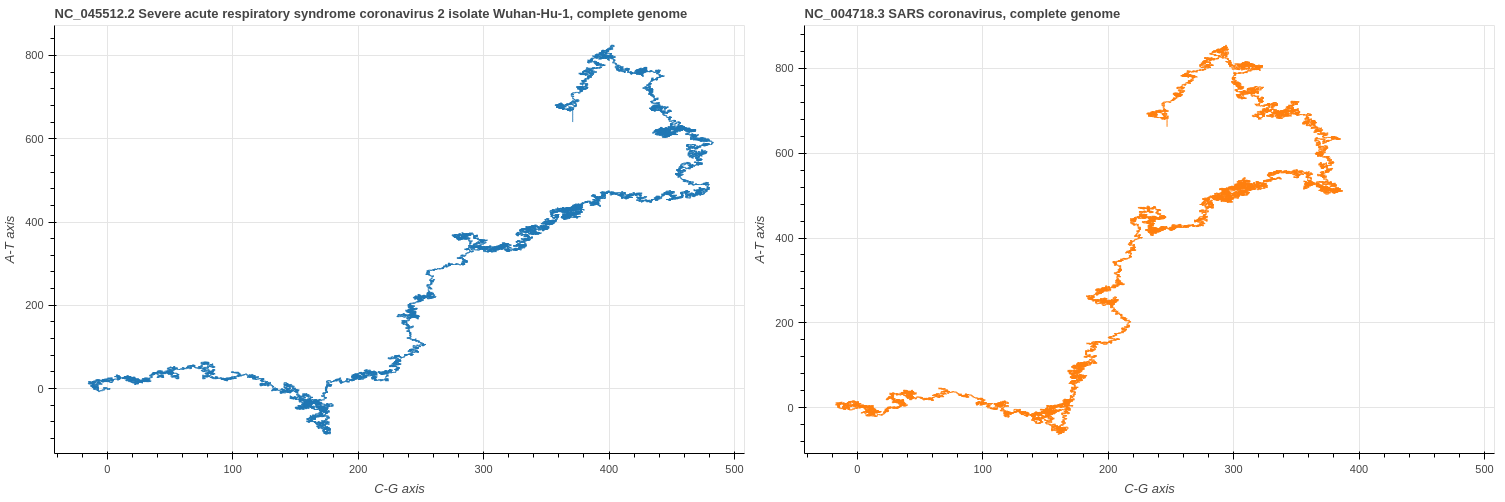
\includegraphics[width=1\textwidth]{figures/comprasion.png}
	\caption{Porovnanie genómov SARS-CoV-2 (zľava) a SARS-CoV (sprava) pomocou Gatesovej metódy.\label{o:latex_friendly_zone}}
\end{figure}

Ako je zrejmé z poskytnutého grafu, obidva vírusy sa navzájom podobajú z hľadiska štruktúry nukleotidovej sekvencie \cite{2d}.

Po spracovaní sekvencií oboch vírusov pomocou algoritmu pairwise2 sa percento podobnosti medzi nimi rovná 83,34\%.

Algoritmus PairWise je variantou najlepšieho algoritmu lokálneho zarovnania Smithovho-Watermanovho algoritmu \cite{pairwise}.
Všetky tieto algoritmy patria do triedy známej ako algoritmy minimálnej úpravy reťazcov.
Bol vybraný na porovnanie sekvencií kvôli spôsobu, akým zarovnáva sekvencie.
Hlavné rozdiely medzi PairWise a iným algoritmom zarovnania sú v tom, že okrem bežných trestov, ako sú Gap Opening Penalty (GOP), Gap Extension Penalty (GEP) a Match, PairWise predstavil dva nové ďalšie parametre použité pre porovnanie \cite{pairwise}.

Samotné porovnanie je možné ľahko vykonať pomocou knižnice BioPython, ako je to demonštrované v priloženom kóde.
\begin{lstlisting}[language=Python, caption=Algoritmus Pairwise2 využívajúci BioPython; COV1.seq a COV2.seq sú sekvencie DNA vírusov SARS-CoV a SARS-CoV-2. Poskytujú sa dva argumenty samotného zarovnania aby sa znížila komlexita a čas zosúladenia.]
    from Bio import pairwise2

    alm = pairwise2.align.globalxx(COV1.seq, COV2.seq,
                 one_alignment_only=True, score_only=True)
    print('Similarity (%):', alm / len(COV2.seq) * 100)
\end{lstlisting}

Najdôležitejšou nevýhodou Gatesovej metódy je však degenerácia, čo znamená, že vizualizácia nemusí byť nevyhnutne jedinečná.
Napríklad TGAC je štvorec (hore, doprava, dole a vľavo), ale rovnako je tomu aj v GTCA (vpravo, hore, vľavo, dole) a obe sekvencie budú mať vo vizualizačnom grafe rovnakú štruktúru.

\subsection{Metóda 2D Matrix}
Ďalšou zaujímavou metódou na vizualizáciu DNA, ktorá pracuje na sekvencii DNA, je metóda 2D matice.
Cieľom je vykresliť celú sekvenciu genómu do štvorcového obrázka s preddefinovanou veľkosťou.
Plotovanie sa vykonáva z ľavého rohu do pravého rohu až po koniec čiary a potom sa presunie na ľavú stranu nového (obr. 2.8).

Každý nukleotid je reprezentovaný pixelom (štvorcom) konkrétnej farby.
\begin{figure}[!ht]
	\centering
	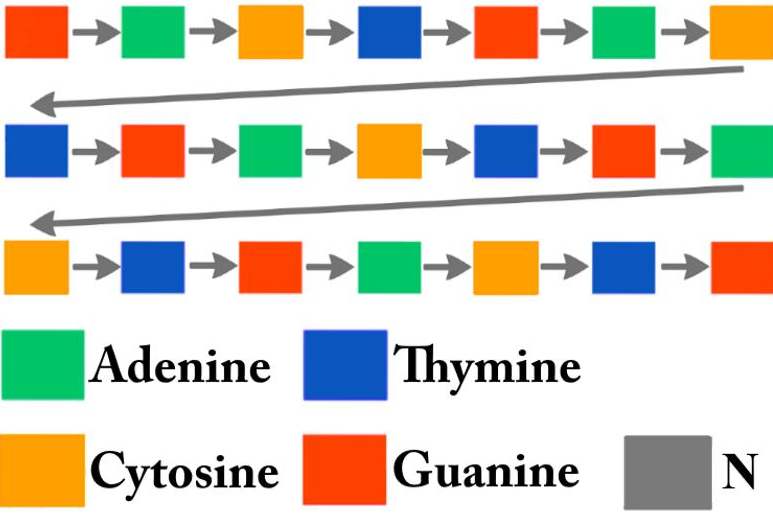
\includegraphics[width=.4\textwidth]{figures/2d.png}
	\caption{Zakreslenie DNA do dvojrozmernej matice.\label{o:latex_friendly_zone}}
\end{figure}

Táto metóda by mohla byť užitočná pri hľadaní tandemových opakovaní \cite{fgene} bez podrobného preskúmania strojom, pretože by mohli byť vizuálne zistiteľné.
Ako je však viditeľné na obrázku 2.9, pre genóm SARS-CoV-2 nie sú nevyhnutné žiadne významné a zrejmé tandemové opakovania.
Dá sa to vysvetliť celkovou malou veľkosťou a zložitosťou genómu.

\begin{figure}[!ht]
	\centering
	
\includegraphics[width=0.7\textwidth]{figures/matrix.png}
	\caption{Vizualizácia genómu SARS-CoV-2 pomocou metódy 2D Matrix. Najplynulejšia sekvencia genómu je zložená z 29 903 nukleotidov a zobrazená matica obsahuje 29 929 pozícií (173 na každej strane), čierne štvorčeky v pravom dolnom rohu predstavujú prázdny priestor, ktorý sa nepoužil na vizualizáciu..\label{o:latex_friendly_zone}}
\end{figure}

Okrem toho táto metóda vykresľuje každý genóm na obrázku pevnej veľkosti, ktorý by sa mohol použiť na jednoznačnú identifikáciu samotnej sekvencie.
Avšak v prípade bodových alebo dokonca významných mutácií môže byť rozdiel v vynesenom genóme ťažko odlíšiteľný bez strojového vyšetrenia.

\subsection{Vylepšenie metódy 2D Matrix}
Táto práca navrhuje novú vizualizačnú techniku, ktorá je schopná vizualizovať každý genóm jedinečne pomocou hash-funkcie \cite{hash}, čo by mohlo byť riešením vyššie uvedenej nevýhody.

Hlavnou myšlienkou vizualizačnej techniky je rekurzívny algoritmus, ktorý rozdeľuje obraz na menšie časti a farbí každú z nich v závislosti na predchádzajucej.
Toto zabráni náhodnému šumu, ktorý by sa mohol objaviť, rozdelením na malé kúsky a samostatným vyfarbením každého z nich.
Namiesto toho existujú väčšie regióny, ktoré si zachovávajú určitú kontinuitu, aj keď sa ich základné časti rozchádzajú.

Rekurzívny algoritmus sa skladá z troch funkcií:
\begin{itemize}
    \item Funkcia, ktorá dosahuje hash nukleotidovej sekvencie pomocou algoritmu sha256 \cite{hash2}.
    \item Funkcia, ktorá rekurzívne rozdelí počiatočný prázdny obrázok na 1/8 častí.
    Pre každú z počiatočných oblastí sa to robí rekurzívne 8-krát.
    \item Funkcia, ktorá zafarbí každú časť podľa hashu a vloží každú časť nad väčšú.
    Parameter nepriehľadnosti je vypočítaný pre každú veľkosť oddielu a slúži na zabránenie prekrývania medzi farbami menších oddielov a väčších (ktoré sú predtým zafarbené).
\end{itemize}

Zoznam 2.5 ukazuje výstup z konzoly počas vytvárania obrázka s veľkosťou 512x512 pixelov.
Hodnoty šírky a výšky predstavujú veľkosť rozdelených obrázkov, ktoré sú zafarbené, a hodnota krytia zobrazuje krytie počas každého prekrytia oddielu.
Obrázky generované na ilustráciu tejto metódy používali rovnicu krytia definovanú ako:\\
\[opacity = 256 * (level / 2) / 2 ^ {(level - 1)}\]
kde úroveň predstavuje súčasnú hĺbku rekurzie. 
Túto rovnicu je však možné zmeniť tak, aby predstavovala ďalšie schémy vyfarbovania.

\begin{lstlisting}[caption=Výstup z konzoly vyrobený počas vizualizácie pomocou vylepšenej metódy 2D Matrix.]
    seed: 223dd4d5c80b98e69f9f8536afa54b...
    width, height: 256.0, 256.0
    opacity: 50%
    width, height: 128.0, 64.0
    opacity: 37%
    width, height: 32.0, 32.0
    opacity: 25%
    width, height: 16.0, 8.0
    opacity: 15%
    width, height: 4.0, 4.0
    opacity: 9%
    width, height: 2.0, 1.0
    opacity: 5%
\end{lstlisting}

Ako je viditeľné na obrázku 2.10, táto metóda umožňuje jednoduché rozlíšenie rôznych genómov voľným okom.

\begin{figure}[!ht]
	\centering
	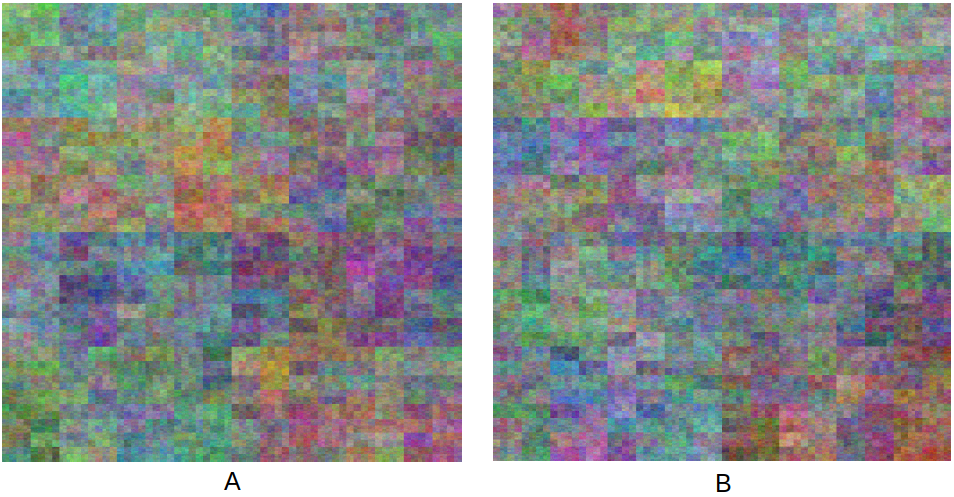
\includegraphics[width=1\textwidth]{figures/2dim.png}
	\caption{Vizualizácia pôvodného genómu SARS-CoV-2 [A] a rovnakého genómu s bodovou mutáciou [B] na druhom nukleotide (T zmenené na G) pomocou vylepšenej metódy 2D Matrix.\label{o:latex_friendly_zone}}
\end{figure}

Kvôli rekurzívnej povahe algoritmu môže byť obraz generovaný v menších alebo väčších veľkostiach a pri zachovaní rovnakej úrovne detailov.

Medzi hlavné nevýhody však patrí malé praktické využitie a obmedzenie týkajúce sa veľkosti genómu.
V súčasnosti metóda podporuje vizualizáciu genómov, ktoré majú menej ako 262 145 nukleotidov kvôli začiatočným rôzmeram obazku (512x512 px).

\subsection{Získanie aminokyselín}

Pre ďalšiu vizualizáciu musí byť surová sekvencia DNA prevedená na sekvenciu aminokyselín.
Existuje 61 kodónov (trinukleotidov) pre 20 aminokyselín a každý z nich je „načítaný“, aby určil určitú aminokyselinu z 20, ktoré sa bežne nachádzajú v bielkovinách.
Každá aminokyselina môže byť napísaná ako písmeno latinskej abecedy.
Preto je sekvencia aminokyselín predstavovaná sekvenciou písmen A-V.

Jeden kodón, AUG, špecifikuje aminokyselinu metionín a tiež slúži ako štartovací kodón na signalizáciu začiatku stavby proteínu.
Existujú ďalšie tri kodóny, ktoré nešpecifikujú aminokyseliny: UAA, UAG a UGA, ktoré povedia bunke, keď je polypeptid kompletný \cite{aminouag}.
Celkovo sa táto zbierka vzťahov kodón-aminokyselina nazýva \textit{genetický kód}, pretože umožňuje bunkám „dekódovať“ mRNA do reťazca aminokyselín.

Pred konverziou sekvencie DNA na aminokyselinu je potrebné ju najskôr transkribovať do molekuly mRNA \cite{rnaseqexp} pomocou funkcie transkripcie ().
Našťastie s funkciou translate () BioPython prevádza mRNA na aminokyselinové reťazce (zdrojový kod 2.5).
Reťazce sú oddelené znakom *, čo je stop kodón (UAA, UAG a UGA).

\begin{lstlisting}[language=Python, caption=Prepis a preklad pomocou BioPythonu]
    cov_DNA = covid19.seq
    cov_mRNA = covid_DNA.transcribe()
    cov_aa = covid_mRNA.translate()
\end{lstlisting}

Som zistil, že genóm SARS-CoV-2 obsahuje 9967 aminokyselín oddelených stop kodónmi * alebo, inými slovami, 775 aminokyselinových reťazcov.
Je potrebné spomenúť, že nie všetky aminokyselinové sekvencie sú bielkoviny.
Iba sekvencie s viac ako 20 aminokyselinami kódujú funkčné proteíny \cite{cov1}.
Krátke aminokyselinové sekvencie sú oligopeptidy a majú ďalšie funkčné skupiny.
Ďalším krokom je filtrovanie získaných sekvencií takým spôsobom, že zostanú len tie dlhé, aby sa sústredili iba na proteíny.

Po odstránení krátkych proteínov iba 5 zvyšných proteínov spĺňa podmienku dĺžky (zdrojový kód 2.6) a sú uvedené v tabuľke 2.1.

Najjednoduchší spôsob overenia výsledkov je nájsť proteínové sekvencie, ktoré sú už k dispozícii v databázach a ktoré sú najviac podobné získaným proteínovým sekvenciám.
Na tieto účely sa použilo vyhľadávanie BLAST.

BLAST (základný vyhľadávací nástroj na lokálne zarovnanie) je algoritmus a program na porovnanie informácií o primárnych biologických sekvenciách, ako sú napríklad aminokyselinové sekvencie proteínov alebo nukleotidy sekvencií DNA a / alebo RNA.
Vyhľadávanie BLAST umožňuje porovnať predmetnú proteínovú alebo nukleotidovú sekvenciu (nazývanú dopyt) s knižnicou alebo databázou sekvencií a identifikovať sekvencie knižnice, ktoré sa podobajú dopytovanej sekvencii nad určitou hranicou.

\begin{lstlisting}[language=Python, caption=Filtrovanie aminokyselinových sekvencií a ich ukladanie do dátového rámca]
    Proteins = covid_aa.split('*')

    #Remove porteins with less than than 50 amino acids
    for i in Proteins[:]:
        if len(i) < 50:
            Proteins.remove(i)
    #Store the protein sequences in a pandas dataframe

    proteins=pd.DataFrame(Proteins)
    proteins['amino acid sequence'] = proteinas[0].apply(str)
    proteins['Protein length'] = proteinas[0].apply(len)
    proteins.rename(columns={0: "sequence"}, inplace=True)
    pro=proteins.drop('sequence', axis=1)
    pro=pro.sort_values(by=['Protein length'], ascending=False)
\end{lstlisting}

\begin{table}[]
    \caption{Získané proteínové sekvencie genómu SARS-CoV-2, ktoré sú zložené z viac ako 50 aminokyselín.}\label{t:1}
	\smallskip
	\centering
    
    \begin{tabular}{|l|l|c|}
    \hline
    \textbf{ } & \textbf{Aminoacid sequence}                                                     & \multicolumn{1}{l|}{\textbf{Protein length}} \\ \hline
    \textbf{1} & CTIVFKRVCGVSAARLTPCGTGTSTDVVYRAFDIYND... & 2701                                         \\ \hline
    \textbf{2} & ASAQRSQITLHINELMDLFMRIFTIGTVTLKQGEIKD... & 290                                          \\ \hline
    \textbf{3} & TNMKIILFLALITLATCELYHYQECVRGTTVLLKEPC... & 123                                          \\ \hline
    \textbf{4} & AQADEYELMYSFVSEETGTLIVNSVLLFLAFVVFLLV... & 83                                           \\ \hline
    \textbf{5} & QQMFHLVDFQVTIAEILLIIMRTFKVSIWNLDYIINL... & 63                                           \\ \hline
    \end{tabular}
\end{table}

Po vyhľadaní reťazca 83 aminokyselín pomocou BLAST výsledky ukázali, že má 100\% podobnosť s malým membránovým proteínom Envelope, ktorý patrí do genómu SARS-CoV-2.
Výsledky vykonaných BLAST hľadaní ďalších získaných proteínov sú uvedené v tabuľke 2.2.
Za zmienku stojí, že najvyššia podobnosť sa zistila medzi ostatnými druhmi koronavírusov.

\begin{table}[]
    \caption{Nejaké výsledky porovnania medzi získanými proteínovými sekvenciami SARS-CoV-2 pomocou BLAST.}\label{t:1}
	\smallskip
	\centering
    \begin{tabular}{|c|c|c|c|c|c|}
        \hline
        \multicolumn{1}{|l|}{}             & \multicolumn{1}{l|}{\textbf{\begin{tabular}[c]{@{}l@{}}Dĺžka \\ proteinu\end{tabular}}} & \multicolumn{1}{l|}{\textbf{DB:ID}} & \multicolumn{1}{l|}{\textbf{Organism}}                                                                  & \multicolumn{1}{l|}{\textbf{Protein}}                                                                  & \multicolumn{1}{l|}{\textbf{Zhoda}} \\ \hline
        \multicolumn{1}{|c|}{\textbf{1}} & \multicolumn{1}{c|}{2701}                                                              & \multicolumn{1}{c|}{P0C6X7}        & \multicolumn{1}{c|}{\begin{tabular}[c]{@{}c@{}}Replicase \\ polyprotein \\ 1ab\end{tabular}}           & \multicolumn{1}{c|}{\begin{tabular}[c]{@{}c@{}}Replicase \\ polyprotein \\ 1ab\end{tabular}}          & \multicolumn{1}{c|}{96\%}           \\ \hline
        \multicolumn{1}{|c|}{\textbf{2}} & \multicolumn{1}{c|}{290}                                                               & \multicolumn{1}{c|}{Q0Q474}        & \multicolumn{1}{c|}{\begin{tabular}[c]{@{}c@{}}Bat \\ coronavirus \\ 279/2005 \\ (BtCoV)\end{tabular}} & \multicolumn{1}{c|}{Protein 3}                                                                        & \multicolumn{1}{c|}{75\%}           \\ \hline
        \multicolumn{1}{|c|}{\textbf{3}} & \multicolumn{1}{c|}{123}                                                               & \multicolumn{1}{c|}{Q3I5J0}        & \multicolumn{1}{c|}{\begin{tabular}[c]{@{}c@{}}Bat \\ coronavirus \\ Rp3/2004\end{tabular}}            & \multicolumn{1}{c|}{Protein 7a}                                                                       & \multicolumn{1}{c|}{89\%}           \\ \hline
        \multicolumn{1}{|c|}{\textbf{4}} & \multicolumn{1}{c|}{83}                                                                & \multicolumn{1}{c|}{P0DTC4}        & \multicolumn{1}{c|}{\begin{tabular}[c]{@{}c@{}}Human SARS \\ coronavirus \\ (SARS-CoV-2)\end{tabular}} & \multicolumn{1}{c|}{\begin{tabular}[c]{@{}c@{}}Envelope \\ small \\ membrane \\ protein\end{tabular}} & \multicolumn{1}{c|}{100\%}          \\ \hline
        \multicolumn{1}{|c|}{\textbf{5}} & \multicolumn{1}{c|}{63}                                                                & \multicolumn{1}{c|}{Q3I5J1}        & \multicolumn{1}{c|}{\begin{tabular}[c]{@{}c@{}}Bat \\ coronavirus \\ Rp3/2004\end{tabular}}            & \multicolumn{1}{c|}{\begin{tabular}[c]{@{}c@{}}Non-\\ structural \\ protein 6\end{tabular}}           & \multicolumn{1}{c|}{69\%}           \\ \hline
        \end{tabular}
\end{table}

\subsection{Identifikácia a vizualizácia ORF}
Ďalšia vizualizácia pracuje s predspracovanými údajmi uloženými v súbore anotácií GenBank.
Ako bolo spomenuté v prvej kapitole tejto práce, skenovanie ORF nie je úplným dôkazom nájdenia génových polôh, pretože nie každý ORF je génovým začiatkom.
Čím je však ORF dlhší, tým je pravdepodobné, že je súčasťou génu. \cite{orf}

Identifikácia kódujúcich sekvencií (CDS) je dôležitým krokom vo funkčnej anotácii génov.
Typický CDS začína ATG a končí stop kodónom.
CDS je sekvencia nukleotidov, ktorá zodpovedá sekvencii aminokyselín v proteíne \cite{bioinformatics}.
Preto bola na identifikáciu kódujúcich oblastí genómu nevyhnutná analýza a získanie aminokyselín (vykonané v časti 2.2.5).
Genóm SARS-CoV-2 kóduje až 50 neštrukturálnych, štrukturálnych a doplnkových proteínov \cite{cov2gene}.

Zdrojový kód 2.7 je výstupný skript pre vizualizáciu, ktorý nájde ORF v genóme SARS-CoV-2 pomocou anotačného súboru genómu.
Minimálna dĺžka proteínu je nastavená na 200 aminokyselín, aby sa získali iba dlhé ORF.

\begin{lstlisting}[caption=Pozície CDS genómu SARS-CoV-2]
    PKGKMESLVPGFNEKTH...FAV - length 4409, strand 1, 253:13483
    CTIVFKRVCGVSAARLT...VNN - length 2701, strand 1, 13449:21555
    LEKTTELLFLVMFLLTT...HYT - length 1293, strand 1, 21502:25384
    ASAQRSQITLHINELMD...VPL - length 290, strand 1, 25347:26220
    SSGLNELNIILVFLFGT...LVQ - length 243, strand 1, 26459:27191
    RSCCFRFHLNEQTKMSD...TQA - length 433, strand 1, 28231:29533
\end{lstlisting}

Som zistil, že genóm Covid-19 má 6 ORF s viac ako 200 aminokyselinami. Obrázok 2.11 ukazuje všetky ORF a CDS načítané z genómu SARS-CoV-2 pomocou BioPython.

\begin{figure}[!ht]
	\centering
	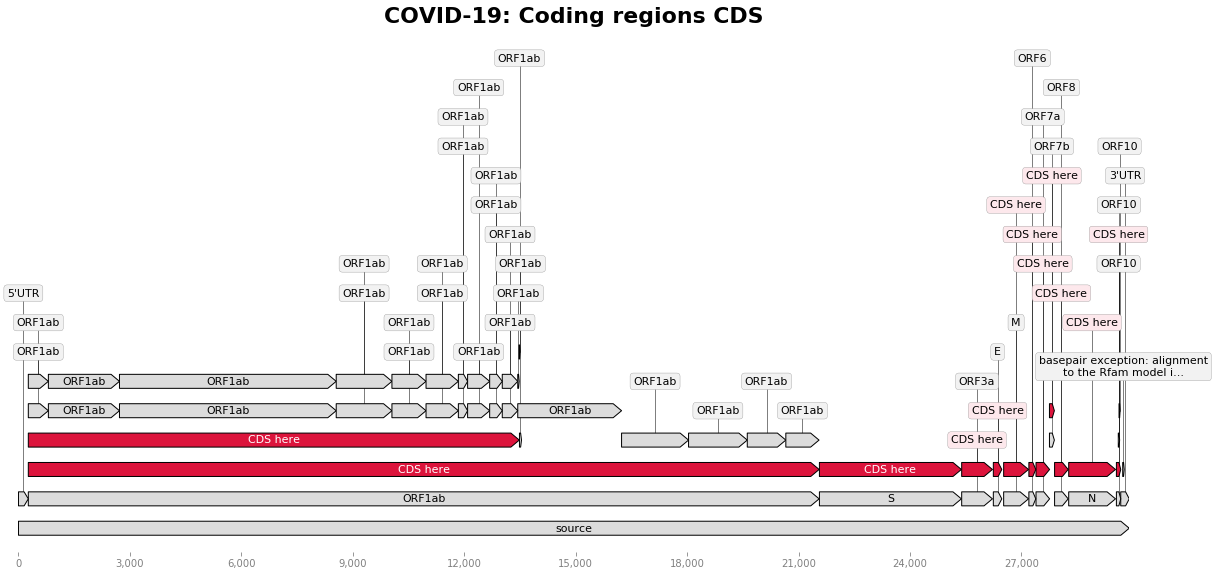
\includegraphics[width=1\textwidth]{figures/cds.png}
	\caption{Kódujúce oblasti genómu SARS-CoV-2 sú medzi ostatnými ORF zvýraznené červenou farbou. Zahŕňajú ORF1ab, ORF3a, S proteín, M proteín a N proteín. Vizualizácia sa vykonáva pomocou programu BioPython\label{o:latex_friendly_zone}}
\end{figure}

Výsledky porovnania získaných sekvencií s existujúcimi sekvenciami sa uskutočňujú pomocou programu BLAST a sú uvedené v tabuľke 2.3.

\begin{table}[]
    \caption{Nejaké výsledky BLAST vyhľadávania pre ORF SARS-CoV-2.}\label{t:1}
	\smallskip
	\centering

    \begin{tabular}{|c|c|c|c|c|c|}
    \hline
               & \textbf{\begin{tabular}[c]{@{}c@{}}Dĺžka\\ ORF\end{tabular}} & \textbf{DB:ID} & \textbf{Protein}                                                        & \textbf{Organism}                                                                 & \textbf{Zhoda} \\ \hline
    \textbf{1} & 4409                                                          & P0C6U8         & \begin{tabular}[c]{@{}c@{}}Replicase\\ polyprotein \\ 1a\end{tabular}   & \begin{tabular}[c]{@{}c@{}}Human \\ SARS\\ coronavirus \\ (SARS-CoV)\end{tabular} & 80\%           \\ \hline
    \textbf{2} & 2701                                                          & P0C6X7         & \begin{tabular}[c]{@{}c@{}}Replicase \\ polyprotein \\ 1ab\end{tabular} & \begin{tabular}[c]{@{}c@{}}Human \\ SARS\\ coronavirus \\ (SARS-CoV)\end{tabular} & 96\%           \\ \hline
    \textbf{3} & 1293                                                          & P59594         & \begin{tabular}[c]{@{}c@{}}Spike\\ glycoprotein\end{tabular}            & \begin{tabular}[c]{@{}c@{}}Human \\ SARS\\ coronavirus \\ (SARS-CoV)\end{tabular} & 76\%           \\ \hline
    \textbf{4} & 290                                                           & Q0Q474         & Protein 3                                                               & \begin{tabular}[c]{@{}c@{}}Bat\\ coronavirus\\ Rp3/2004\end{tabular}              & 95\%           \\ \hline
    \textbf{5} & 243                                                           & Q0Q472         & \begin{tabular}[c]{@{}c@{}}Membrane\\ protein\end{tabular}              & \begin{tabular}[c]{@{}c@{}}Bat\\ coronavirus\\ Rp3/2004\end{tabular}              & 92\%           \\ \hline
    \textbf{6} & 433                                                           & P59595         & \begin{tabular}[c]{@{}c@{}}Nucleoprotein\\ N\end{tabular}               & \begin{tabular}[c]{@{}c@{}}Human \\ SARS\\ coronavirus \\ (SARS-CoV)\end{tabular} & 91\%           \\ \hline
    \end{tabular}
\end{table}

\section{Zostavenie softvéru}
Softvér vyvinutý v priebehu tejto práce sa javí ako zhrnutie kodu použítého na vizualizáciu genómu SARS-CoV-2 v skôr opísaných metódach a je určený pre platformu Linux.

Program bol vyvinutý a otestovaný na notebooke \textit{ASUS X556UQ}, ktorý ma nasledujúce charakteristiky:
\begin{itemize}
    \item \textit{RAM:} 8 GB
    \item \textit{CPU:} Intel© Core™ i5-6198DU CPU @ 2.30GHz × 2
    \item \textit{Grafická karta:} Nvidia Geforce 940MX
    \item \textit{HDD:} 1 TB
    \item \textit{OS:} Linux Mint 20 Cinnamon (kernel v. 5.4.0-66-generic)
\end{itemize}

Na rozdiel od webových prehľadávačov genómu, kde sa výpočty vykonávajú na strane servera, navrhovaný softvér všeobecne predstavuje samostatnú konzolovú aplikáciu.
Nevykonávajú sa nijaké významné výpočty, a preto aplikácia nespĺňa náročné systémové požiadavky.

Napriek skôr opísaným moderným riešeniam reprezentujúcim údaje o genóme sa tento softvér javí ako jednoduchý vizualizačný nástroj, ktorý nepodporuje rôzne vlastné vizualizačné stopy ani grafické rozhranie.
Nedostatok prispôsobenia možno vysvetliť extrémnou zložitosťou vytvárania plne funkčného prehľadávača genómu.

Vyvinutý softvér je napísaný podľa paradigmy funkčného programovania.
Tento prístup k písaniu softvéru bol zabezpečený predovšetkým nízkou zložitosťou vyvinutého riešenia.

Softvér je napísaný hlavne pomocou balíka BioPython v Pythone 3.8.
Všetky požadované balíčky sú uvedené v projektovej dokumentácii.

Hlavnou myšlienkou programu je umožniť používateľovi zvoliť si, ktoré informácie týkajúce sa genómu vírusu si chce zobraziť.
Vyvinutý softvér podporuje dva režímy expluatácie: \textit{verbose} a \textit{quiet}.

Počas prvého režímu používateľ visualizuje genomy pomocou konzolovej navigácie programu. 
Tento režím poskytuje popis vykonávanych akcíi a umožňuje zadávať požiadované data počas behu programu.

Počas druhého režímu sa ide o využitie programu pomocou argumentov príkazového riadku, čo umožnuje d'alšiu automatizáciu a presmerovanie vystupu.

Program skladá sa z 8 modulov, ktoré majú vlastnú úlohu pri samotnom procese vizualizácie:
\begin{enumerate}
    \item \textbf{Main Module} je jadrom programu. Zodpovedá za zabezpečenie navigácie v rámci programu používateľom.
    Zaoberá sa vstupom a výstupom z konzoly, navrhuje dostupné metódy vizualizácie a získava podrobnosti potrebné na ich výkon.
    \item \textbf{Sequence Collector} je zodpovedný za stiahnutie všetkých požadovaných sekvencií a súborov anotácií z databázy NCBI pre vizualizáciu genómu SARS-CoV-2.
    \item \textbf{Statistics Generator} získava štatistické údaje, ako je obsah GC a distribúcia nukleotidov / aminokyselín.
    Užívateľ si môže zvoliť oblasť genómu, ktorá sa má štatisticky analyzovať.
    \item \textbf{Gates Visualization} vykonáva vizualizáciu pomocou Gatesovej metódy do súboru {\fontfamily{lmtt}\selectfont -Gates.png}.
    Užívateľ je schopný zvoliť oblasť genómu ktorú chce vizualizovať.
    \item \textbf{2D Matrix} modul vykreslí vybraný genóm do 2D matice do súboru .png. Veľkosť výstupného obrázka sa počíta automaticky.
    \item \textbf{2D HMatrix} modul vykreslí genóm do 2D matice vybranej veľkosti pomocou algoritmu hash funkcie do súboru .png.
    \item \textbf{ORF Plotter} generuje obraz distribúcie ORF a pomeru obsahu GC v genóme.
    \item \textbf{Comparison} modul vykonáva porovnanie vybraných genómov. Percento podobnosti sa získa na základe algoritmu pairwise2.
\end{enumerate}

Moduly nie sú schopné vzájomne interagovať, ale každý z nich je využivány s hlavného počas visualizácie.

Každý z modulov je popísaný v dokumentácii a je sprevádzaný príkladmi vstupu a výstupu.
Každý modul navyše obsahuje rôzne run-time testy, ktoré zabraňujú neočakávanému správaniu programu.

V súčasnosti všetky moduly podporujú spracovanie rôznych genómov, pretože výkon týchto metód nezávisí od konkrétnych vlastností genómu.
Neodporúča sa však používať Proteínový plotter s genómami, ktoré kvôli svojej zložitosti obsahujú zložité intrón-exón štruktúry a sú väčšie ako 50000 nukleotidov kvôli extrémnej dĺžke a môžnym chýbam počas vyhľadavaní ORF.
V takom prípade sa výsledky môžu výrazne líšiť od skutočných charakteristík genómu a program bude potrebováť náročné systémové požiadavky.